%%%%%%%%%%%%%%%%%%%%%%%%%%%%%%%%%%%%%%%%%
% A Comprehensive Look at The Empirical Performance of Equity Premium Prediction
% Ivo Welch and Amit Goyal (2008)
% 
%
% Replication Paper
% FIN 7806
% Summer 2019
%
% Daniel Amy
% damy001@fiu.edu
% Florida International University
%
%%%%%%%%%%%%%%%%%%%%%%%%%%%%%%%%%%%%%%%%%

%----------------------------------------------------------------------------------------
%	PACKAGES AND OTHER DOCUMENT CONFIGURATIONS
%----------------------------------------------------------------------------------------

\documentclass[a4paper, 12pt]{article} % Font size (can be 10pt, 11pt or 12pt) and paper size (remove a4paper for US letter paper)

\usepackage[protrusion=true,expansion=true]{microtype} % Better typography
\usepackage{graphicx} % Required for including pictures
\usepackage{wrapfig} % Allows in-line images

\usepackage{mathpazo} % Use the Palatino font
\usepackage[T1]{fontenc} % Required for accented characters
\linespread{1.05} % Change line spacing here, Palatino benefits from a slight increase by default
%---------------------------
\usepackage[utf8]{inputenc}
\usepackage[left=1in,right=1in,top=2cm,bottom=2cm]{geometry}
\usepackage{crop,graphicx,amsmath,array,color,amssymb,flushend,stfloats,amsthm,chngpage,times,fancyhdr,lipsum,lastpage}
\usepackage{indentfirst} % Indents first paragraph after section
\usepackage{natbib}
\usepackage{setspace}

%%%%%%%%%%%%   Header and Footer  %%%%%%%%%%%%%
\pagestyle{fancy}

\fancypagestyle{plain}{%
  \renewcommand{\headrulewidth}{0pt}%
  \fancyhf{}%
  %\fancyfoot[R]{Page \bf\thepage\ \rm of \bf\pageref{LastPage}}%
}
%\pagenumbering{gobble} % Removes page numbers

%--------------------------

\makeatletter
\renewcommand\@biblabel[1]{\textbf{#1.}} % Change the square brackets for each bibliography item from '[1]' to '1.'
\renewcommand{\@listI}{\itemsep=0pt} % Reduce the space between items in the itemize and enumerate environments and the bibliography

\renewcommand{\maketitle}{ % Customize the title - do not edit title and author name here, see the TITLE block below
\begin{flushright} % Right align
{\LARGE\@title} % Increase the font size of the title

\vspace{40pt} % Some vertical space between the title and author name

{\large\@author} % Author name
\\\@date % Date

\vspace{30pt} % Some vertical space between the author block and abstract
\end{flushright}
}

%----------------------------------------------------------------------------------------
%	TITLE
%----------------------------------------------------------------------------------------

\title{\textbf{{{\Large A Comprehensive Look at The Empirical Performance of Equity Premium Prediction}}}\\ % Title
{\normalsize Ivo Welch and Amit Goyal}} % Subtitle

\author{\textsc{Daniel Amy} % Author
\\{\small FIN 7806 - Paper Replication}
\\{\textit{Florida International University}}} % Institution

\date{\today} % Date

%----------------------------------------------------------------------------------------

\begin{document}

\maketitle % Print the title section

%\doublespacing
% or:
%\onehalfspacing

%----------------------------------------------------------------------------------------
%	ABSTRACT AND KEYWORDS
%----------------------------------------------------------------------------------------

%\renewcommand{\abstractname}{Summary} % Uncomment to change the name of the abstract to something else

%\begin{abstract}
%Morbi tempor congue porta. Proin semper, leo vitae faucibus dictum, metus mauris lacinia lorem, ac congue leo felis eu turpis. Sed nec nunc pellentesque, gravida eros at, porttitor ipsum. Praesent consequat urna a lacus lobortis ultrices eget ac metus. In tempus hendrerit rhoncus. Mauris dignissim turpis id sollicitudin lacinia. Praesent libero tellus, fringilla nec ullamcorper at, ultrices id nulla. Phasellus placerat a tellus a malesuada.
%\end{abstract}
%
%\hspace*{3,6mm}\textit{Keywords:} lorem , ipsum , dolor , sit amet , lectus % Keywords
%
%\vspace{30pt} % Some vertical space between the abstract and first section

%----------------------------------------------------------------------------------------
%	ESSAY BODY
%----------------------------------------------------------------------------------------

%----------------------------------------------------------------------------------------
%	ESSAY BODY
%----------------------------------------------------------------------------------------

\section*{Introduction}
\doublespacing

In this paper Hardin and Wu investigate the effects of banking relationships on real estate investment trust (REIT) capital structure. This contribution to REIT literature explores the dramatic increase in the use of bank debt since 1995.

Publicly traded REITs are unique legal entities that own, operate or finance income-producing real estate. Modeled after mutual funds, REITs historically have provided investors of all types regular income streams, diversification and long-term capital appreciation. They provide a means of diversification and liquidity to investors that direct real estate investment cannot provide.

REITs have a limited ability to retain internal cash flows due to required dividend payouts of 90\% of annual taxable income in order to maintain their favored status which is exempt from corporate taxes. Consequently,
they rely heavily on the liquidity provided by banks when making property acquisitions and developing new properties as these transactions typically are too large to be financed by retained earnings.

There has been a dramatic shift in the sources of funds used by REITs over the past twenty years. Mortgages have become a smaller component of the capital structure puzzle. More and more bank debt has been utilized as the preferred method of financing acquisitions. This shift has connected the real estate market more closely with traditional capital markets.

Hardin and Wu address several questions for the first time. They explore if banking relationships influence debt structure and if REITs with banking relationships are more likely to have access to public debt markets. They also examine if strong banking relationships lead to a reduction in the use of secured debt in REIT debt structure as well as effect on overall leverage.

\subsection*{Recent Trends and Legislation}

As REITs have matured over the years they have developed banking relationships through repeated borrowing with the same financial institutions. New sources have capital have developed to supplement traditional mortgage financing. Bank lines of credit, capital market debt, common and preferred equity are all viable funding tools available to modern REITs that are properly positioned.

Umbrella Partnership REITs (UPREIT) legislation in 1993 is often credited with initiating the modern REIT era. This law allowed investors to contribute property in exchange for limited-partnership units that were tax-exempt.

In 1999, the repeal of Glass-Steagall removed major regulatory hurdles limiting the ability of commercial banks to provide investment banking services. 
Commercial banks could now directly underwrite public securities 
and REITs could now gain access to public capital markets based on their lending relationships.

%------------------------------------------------

\section*{Literature and Theoretical Background}

\subsection*{REIT Capital Structure } 
Existing literature on REIT Capital Structure has offered some conflicting results. Howe and Shilling (1988) and Elayan, Meyer and Li (2004) found evidence of signaling behavior through positive stock price reactions to debt offerings and negative reaction to equity issuances. Brown and Riddiough (2003) and Ooi, Ong and Li (2010) provide evidence of long-run debt ratio targeting by REITs that issue public debt in order to maintain investment-grade credit ratings. Market timing behavior is observed when capital structure decisions are made to adjust towards targeted levels. Faulkender and Petersen (2006) find that the source of REIT capital is important. Links are observed that confirm whether firms utilize private or public debt markets influences their debt priority structure. 

\subsection*{Bank Debt and Effects of Banking Relationships}

The transition from secured to unsecured debt is documented by Boot and Thakor (1994). They identify how collateral is useful in the early stages of a banking relationship in mitigating capital market frictions but that REIT collateral requirements are gradually reduced as banking relationships strengthen. This increased access to public debt markets using unsecured debt ultimately results in lower secured debt ratios. Dennis, Nandy and Sharpe (2000) show how informational asymmetries and other capital market frictions between REITs and lenders are reduced allowing for a greater use of more flexible unsecured debt. 

The asset substitution problem is addressed by Brown and Marble (2007) where they find asset substitution decreases in the proportion of the original debt that is secured implying that firms with lower secured debt ratio would also have lower leverage. The rapid growth of the REIT industry has occurred primarily via property acquisitions and mergers. Subsequently, the asset substitution problem is a potential issue for lenders as less secured debt implies more potential risks leading them to impose restrictions through the use of loan covenants to control REIT leverage. They also show how higher leverage may not always be the optimal financing strategy for REITs since there are no tax benefits from borrowing and many REITs have incentives to improve their credit ratings. These factors provide a case supporting the idea that REITs with banking relationships should have lower leverage.

Johnson (1998) offers an alternative theory on REIT leverage by arguing that asymmetric information-related problems lower optimal leverage of firms. REITs that continually borrow from the same banks benefit from stronger banking relationships which would lead to higher leverage for firms with banking relationships as a result of reduced capital market frictions. 

Hardin and Wu observe empirical evidence supporting Brown and Marble (2007) and not Johnson (1998).

%------------------------------------------------

\section*{Data and Preliminary Analysis}

Firms are selected that are listed on the NYSE, AMEX or NASDAQ and have elected REIT tax status at the beginning of the sample year (1992). They must be registered with the National Association of Real Estate Investment Trusts (NAREIT) and be classified as an Equity REIT for inclusion in the sample.

Three data sources are utilized for sample construction:
\begin{enumerate}
\item Loan Pricing Corporation’s (LPC’s) DealScan database
\begin{itemize}
\item 1,434 REIT bank loans are identified from the database (1992-2004)
\end{itemize}
\item SDC Global New Issues database
\begin{itemize}
\item Public debt offerings, which includes 769 nonconvertible REIT public debt offerings
\item Equity offerings, including 885 equity offerings issued between (1992-2004)
\end{itemize}
\item SNL REIT database
\begin{itemize}
\item Provides detailed firm-level information
\end{itemize}
\end{enumerate}

%------------------------------------------------

\section*{Empirical Results}


Hardin and Wu find (Table 3) a positive effect on firms credit ratings for REITs with banking relationships and longer term debt that is statistically significant at the 5\% level. This higher credit rating can then be utilized to issued unsecured public debt offering an explanation for REITs recent reduced reliance on debt secured by mortgages.

Increased use of public debt markets by public REITs for funding has the effect of integrating real estate assets into the broader capital markets. It brings some of level of increased efficiency to a real estate market that is inherently inefficient due to illiquidity and informational asymmetries.

Banking relationships that are strengthened through repeated use appear to be used as a tool for REITs to gain access to debt that is not secured by collateral.

\begin{center}
\textbf{Table 3: Banking relationships and access to the public debt markets}
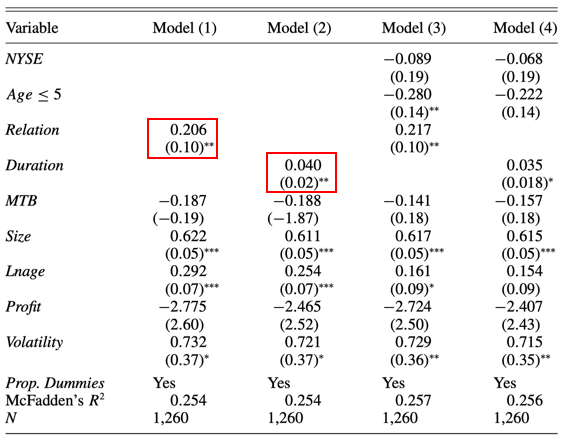
\includegraphics[width=1\textwidth]{Table_III.png}

\end{center}


\begin{center}
\textbf{Table 5: Banking relationships and secured debt ratios (fraction secured)}
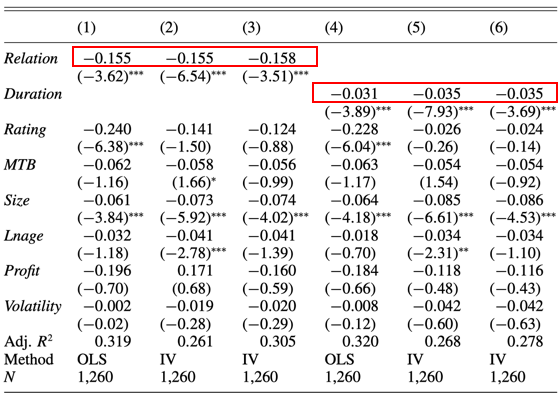
\includegraphics[width=1\textwidth]{Table_V.png}

\end{center}

Table 5 displays results of regressions where the ratio of REITs secured to unsecured debt is the dependent variable. Here Hardin and Wu find a strong negative relation between banking relationships and secured debt ratios. This seems to confirm the theory that stronger relationships have been responsible for the shift from mortgages as a primary funding source for REITs.

\begin{center}
\textbf{Table 7: Banking relationships and market leverage}
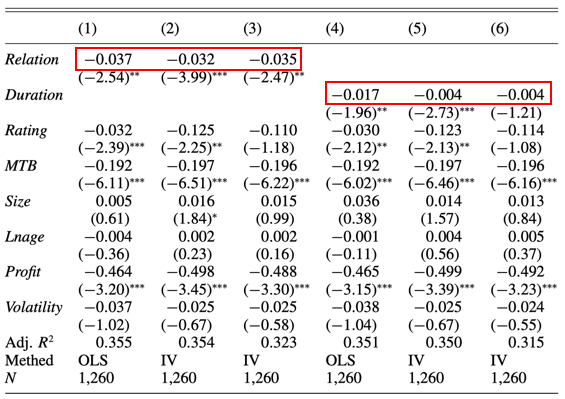
\includegraphics[width=1\textwidth]{Table_VII.png}

\end{center}

An inverse relationship between REIT leverage and banking relationships is observed by the regression results in Table 7 of their findings. This is contrary to the conclusions of Johnson (1998) and supports Brown and Marble's (2007) asset substitution theory. REITs now relying on unsecured debt for new acquisitions must maintain lower leverage ratios in order to obtain loans and maintain investment-grade credit ratings.

\newpage

\begin{center}
\textbf{Table 8: Statistics of REIT public debt, equity and bank loan issuance}
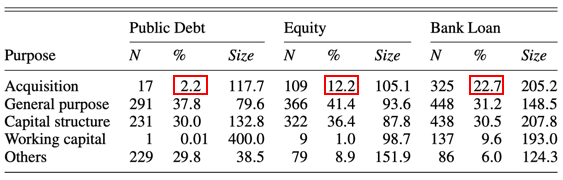
\includegraphics[width=1\textwidth]{Table_VIII.png}

\end{center}

Descriptive statistics are presented in Table 8 that illustrate how REITs have used access to bank funding to reconfigure their liability structures.
Bank loans and equity offerings are most frequently used to fund acquisitions and investment while public debt is seldom used for this purpose. This confirms the findings of Faulkender and Petersen (2006) that the source of funds plays an important role in REIT capital allocation.


%------------------------------------------------

\section*{Key Findings}

Harden and Wu find results indicating that REITs with banking relationships are more likely to have a long-term bond rating and subsequently issue public debt and that these relationships lead to lower secured debt ratios and less use of leverage. Their data also concludes that REITs often use proceeds from bank debt and equity to fund property acquisitions and then issue public securities to reconfigure capital structure. REITs utilize this process as a form of bridge financing.

These findings are important because under traditional capital structure theory a firm with no tax liability would have incentive to be 100\% levered. REITs, however, cannot rely on retained earnings to fully fund new projects efficiently and must maintain a credit rating strong enough to borrow unsecured funds quickly to capitalize on available opportunities. This is only possible if they maintain leverage to a level that is deemed an acceptable amount of risk by lenders.

%------------------------------------------------

\section*{Topics for Further Research}
\subsection*{Are results consistent across all REIT sectors?}
REITs are segmented by investment strategy and asset class. These segments have specific cash flows and associated risks and require different managerial approaches. Hardin and Wu examine the effect of banking relationships on the overall public REIT market. A logical next step would be to investigate if their findings hold when a cross-section of all REIT sectors are studied. Are banking relationships more important to some sectors than others due to factors specific to their underlying collateral or management strategy?

\begin{center}
\textbf{REIT market capitalization}
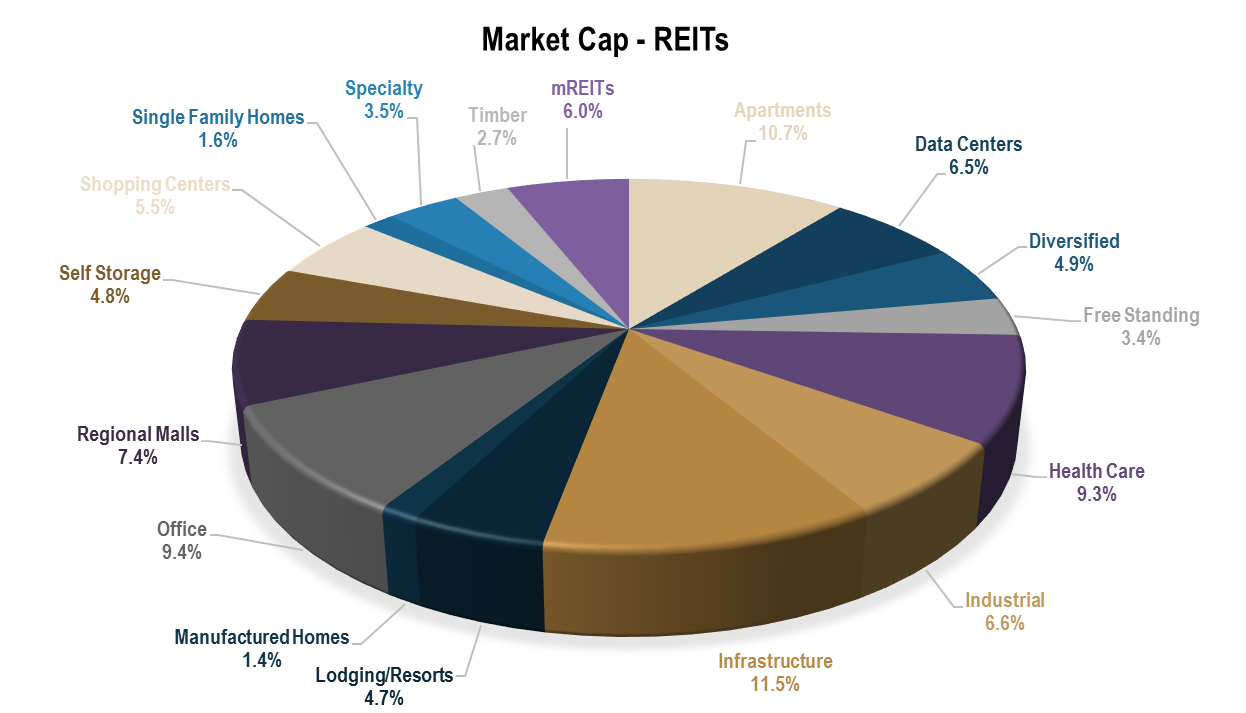
\includegraphics[width=1\textwidth]{REIT.png}

\end{center}


\subsection*{How is REIT capital structure impacted at different phases of the cycle?}


Another next step building on the work of Hardin and Wu would be to identify how REIT debt structure decisions are impacted by phases in the real estate cycle. Real estate assets have a cyclical nature of somewhere between ten to eighteen years depending on the study. Development decisions are impacted by this cycle and new projects are often found to agglomerate around ideal time periods.

Glenn Mueller has identified four phases of the real estate cycle. Commercial real estate cash flows are dependent on rental growth rates and their relationship to inflation. REITs are subject to the same forces as private investors and developers. Thus, their funding needs for acquisitions and development of new projects will vary depending on phase of the cycle. 

Perhaps a new information could be discovered by testing these results at different phases to see how this type of timing influences borrowing patterns and targeted debt ratios. Data collection would be challenging and could require significant time and effort. The field of real estate research is not as mature as corporate finance and reliable data is only be available for the last few complete cycles. Often the phase of the at a particular time is not accurately identified until long after it has completed. Nevertheless, some useful information could be discovered in this area in spite of a small sample size if an appropriate sample is collected.

\begin{center}
\textbf{Real estate cycle}
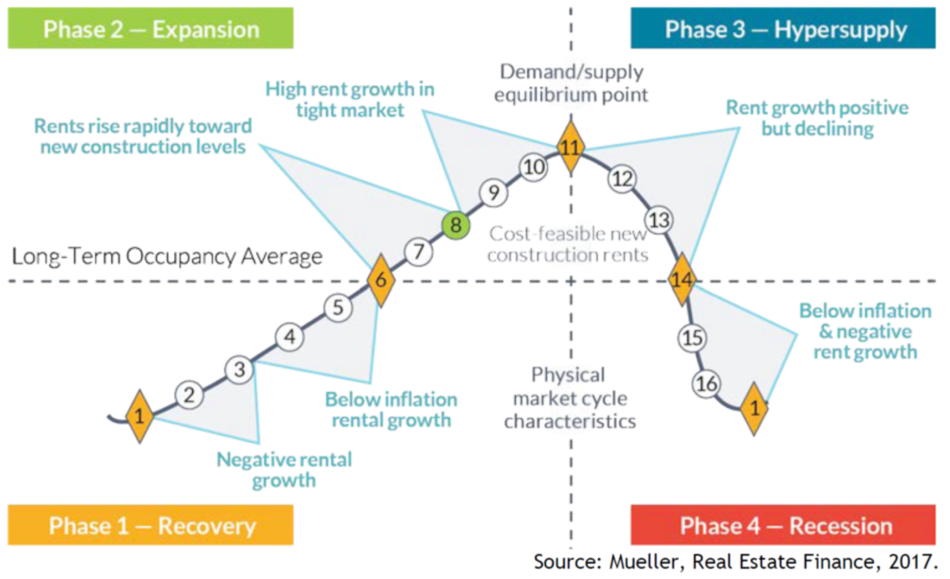
\includegraphics[width=1\textwidth]{recycle.png}

\end{center}
\subsection*{What is the impact on REIT capital structure during crisis?}

Public REITs integration with traditional capital markets exposes them to the market events more than private real estate investment. Extending this research further could lead to an analysis of leverage and banking relationships during times of crisis and how long is needed before equilibrium levels are resumed. \\
\\
\begin{center}
\textbf{MSCI US REIT Index}

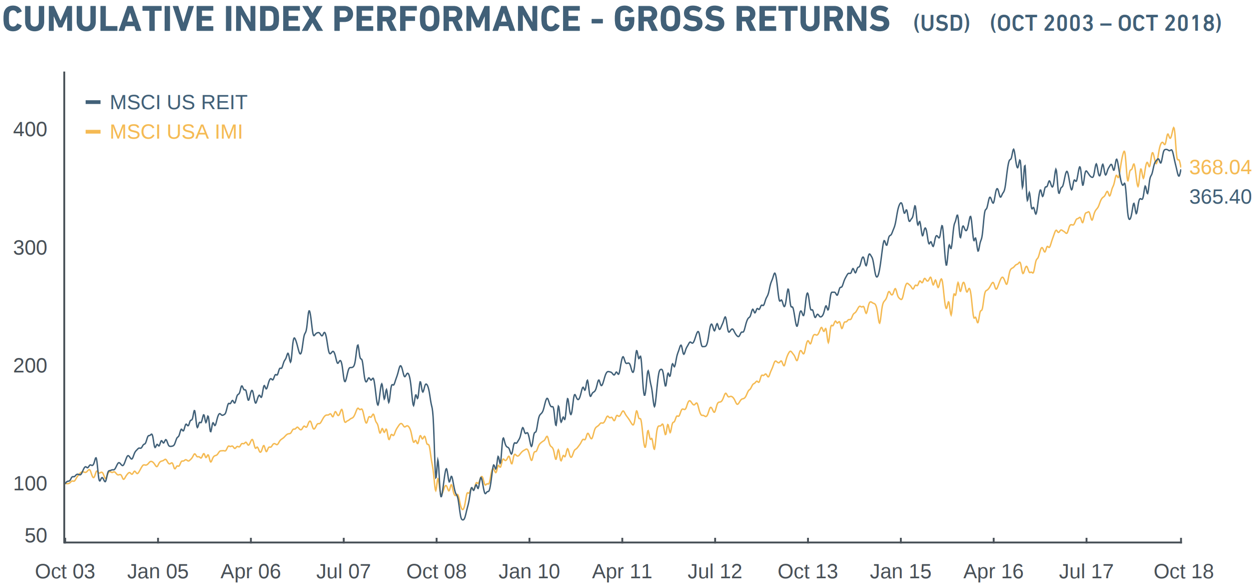
\includegraphics[width=1\textwidth]{msci.png}

\end{center}
\subsection*{Tobin's Q vs MTB}

Hardin and Wu control for market to book value (MTB) in their regression analysis. Tobin's Q is a measure that is often used in place of MTB because it is based on replacement costs instead of book value. Inflation will cause book value to typically be higher than replacement cost causing MTB to be higher than Q as a result. A future study could assess if the results of this paper are significantly affected by a lower measure of valuation.


\begin{itemize}


\item Tobin's Q

$$\frac{Market\: value\: of\: reproducible\: real \:capital\: assets}{Current \:replacement \:cost \:of \:assets}$$

\item Q in real estate

$$\frac{Market\: price\: of\: existing\: real\: estate}{Cost\: of\: land\: + improvements\: construction\: cost}$$

\item Market to Book Ratio (MTB) 

$$\frac{Market\: value\: of\: reproducible\: real \:capital\: assets}{Book\: value}$$

\end{itemize}

%------------------------------------------------
%----------------------------------------------------------------------------------------
%	BIBLIOGRAPHY
%----------------------------------------------------------------------------------------
\clearpage
\fancyhf{}
\bibliographystyle{rusnat}

\bibliography{hardin}
\nocite{*}

%----------------------------------------------------------------------------------------

\end{document}